% Options for packages loaded elsewhere
\PassOptionsToPackage{unicode}{hyperref}
\PassOptionsToPackage{hyphens}{url}
\PassOptionsToPackage{dvipsnames,svgnames,x11names}{xcolor}
%
\documentclass[
  letterpaper,
  DIV=11,
  numbers=noendperiod]{scrartcl}

\usepackage{amsmath,amssymb}
\usepackage{lmodern}
\usepackage{iftex}
\ifPDFTeX
  \usepackage[T1]{fontenc}
  \usepackage[utf8]{inputenc}
  \usepackage{textcomp} % provide euro and other symbols
\else % if luatex or xetex
  \usepackage{unicode-math}
  \defaultfontfeatures{Scale=MatchLowercase}
  \defaultfontfeatures[\rmfamily]{Ligatures=TeX,Scale=1}
\fi
% Use upquote if available, for straight quotes in verbatim environments
\IfFileExists{upquote.sty}{\usepackage{upquote}}{}
\IfFileExists{microtype.sty}{% use microtype if available
  \usepackage[]{microtype}
  \UseMicrotypeSet[protrusion]{basicmath} % disable protrusion for tt fonts
}{}
\makeatletter
\@ifundefined{KOMAClassName}{% if non-KOMA class
  \IfFileExists{parskip.sty}{%
    \usepackage{parskip}
  }{% else
    \setlength{\parindent}{0pt}
    \setlength{\parskip}{6pt plus 2pt minus 1pt}}
}{% if KOMA class
  \KOMAoptions{parskip=half}}
\makeatother
\usepackage{xcolor}
\setlength{\emergencystretch}{3em} % prevent overfull lines
\setcounter{secnumdepth}{-\maxdimen} % remove section numbering
% Make \paragraph and \subparagraph free-standing
\ifx\paragraph\undefined\else
  \let\oldparagraph\paragraph
  \renewcommand{\paragraph}[1]{\oldparagraph{#1}\mbox{}}
\fi
\ifx\subparagraph\undefined\else
  \let\oldsubparagraph\subparagraph
  \renewcommand{\subparagraph}[1]{\oldsubparagraph{#1}\mbox{}}
\fi

\usepackage{color}
\usepackage{fancyvrb}
\newcommand{\VerbBar}{|}
\newcommand{\VERB}{\Verb[commandchars=\\\{\}]}
\DefineVerbatimEnvironment{Highlighting}{Verbatim}{commandchars=\\\{\}}
% Add ',fontsize=\small' for more characters per line
\usepackage{framed}
\definecolor{shadecolor}{RGB}{241,243,245}
\newenvironment{Shaded}{\begin{snugshade}}{\end{snugshade}}
\newcommand{\AlertTok}[1]{\textcolor[rgb]{0.68,0.00,0.00}{#1}}
\newcommand{\AnnotationTok}[1]{\textcolor[rgb]{0.37,0.37,0.37}{#1}}
\newcommand{\AttributeTok}[1]{\textcolor[rgb]{0.40,0.45,0.13}{#1}}
\newcommand{\BaseNTok}[1]{\textcolor[rgb]{0.68,0.00,0.00}{#1}}
\newcommand{\BuiltInTok}[1]{\textcolor[rgb]{0.00,0.23,0.31}{#1}}
\newcommand{\CharTok}[1]{\textcolor[rgb]{0.13,0.47,0.30}{#1}}
\newcommand{\CommentTok}[1]{\textcolor[rgb]{0.37,0.37,0.37}{#1}}
\newcommand{\CommentVarTok}[1]{\textcolor[rgb]{0.37,0.37,0.37}{\textit{#1}}}
\newcommand{\ConstantTok}[1]{\textcolor[rgb]{0.56,0.35,0.01}{#1}}
\newcommand{\ControlFlowTok}[1]{\textcolor[rgb]{0.00,0.23,0.31}{#1}}
\newcommand{\DataTypeTok}[1]{\textcolor[rgb]{0.68,0.00,0.00}{#1}}
\newcommand{\DecValTok}[1]{\textcolor[rgb]{0.68,0.00,0.00}{#1}}
\newcommand{\DocumentationTok}[1]{\textcolor[rgb]{0.37,0.37,0.37}{\textit{#1}}}
\newcommand{\ErrorTok}[1]{\textcolor[rgb]{0.68,0.00,0.00}{#1}}
\newcommand{\ExtensionTok}[1]{\textcolor[rgb]{0.00,0.23,0.31}{#1}}
\newcommand{\FloatTok}[1]{\textcolor[rgb]{0.68,0.00,0.00}{#1}}
\newcommand{\FunctionTok}[1]{\textcolor[rgb]{0.28,0.35,0.67}{#1}}
\newcommand{\ImportTok}[1]{\textcolor[rgb]{0.00,0.46,0.62}{#1}}
\newcommand{\InformationTok}[1]{\textcolor[rgb]{0.37,0.37,0.37}{#1}}
\newcommand{\KeywordTok}[1]{\textcolor[rgb]{0.00,0.23,0.31}{#1}}
\newcommand{\NormalTok}[1]{\textcolor[rgb]{0.00,0.23,0.31}{#1}}
\newcommand{\OperatorTok}[1]{\textcolor[rgb]{0.37,0.37,0.37}{#1}}
\newcommand{\OtherTok}[1]{\textcolor[rgb]{0.00,0.23,0.31}{#1}}
\newcommand{\PreprocessorTok}[1]{\textcolor[rgb]{0.68,0.00,0.00}{#1}}
\newcommand{\RegionMarkerTok}[1]{\textcolor[rgb]{0.00,0.23,0.31}{#1}}
\newcommand{\SpecialCharTok}[1]{\textcolor[rgb]{0.37,0.37,0.37}{#1}}
\newcommand{\SpecialStringTok}[1]{\textcolor[rgb]{0.13,0.47,0.30}{#1}}
\newcommand{\StringTok}[1]{\textcolor[rgb]{0.13,0.47,0.30}{#1}}
\newcommand{\VariableTok}[1]{\textcolor[rgb]{0.07,0.07,0.07}{#1}}
\newcommand{\VerbatimStringTok}[1]{\textcolor[rgb]{0.13,0.47,0.30}{#1}}
\newcommand{\WarningTok}[1]{\textcolor[rgb]{0.37,0.37,0.37}{\textit{#1}}}

\providecommand{\tightlist}{%
  \setlength{\itemsep}{0pt}\setlength{\parskip}{0pt}}\usepackage{longtable,booktabs,array}
\usepackage{calc} % for calculating minipage widths
% Correct order of tables after \paragraph or \subparagraph
\usepackage{etoolbox}
\makeatletter
\patchcmd\longtable{\par}{\if@noskipsec\mbox{}\fi\par}{}{}
\makeatother
% Allow footnotes in longtable head/foot
\IfFileExists{footnotehyper.sty}{\usepackage{footnotehyper}}{\usepackage{footnote}}
\makesavenoteenv{longtable}
\usepackage{graphicx}
\makeatletter
\def\maxwidth{\ifdim\Gin@nat@width>\linewidth\linewidth\else\Gin@nat@width\fi}
\def\maxheight{\ifdim\Gin@nat@height>\textheight\textheight\else\Gin@nat@height\fi}
\makeatother
% Scale images if necessary, so that they will not overflow the page
% margins by default, and it is still possible to overwrite the defaults
% using explicit options in \includegraphics[width, height, ...]{}
\setkeys{Gin}{width=\maxwidth,height=\maxheight,keepaspectratio}
% Set default figure placement to htbp
\makeatletter
\def\fps@figure{htbp}
\makeatother

\KOMAoption{captions}{tableheading}
\makeatletter
\makeatother
\makeatletter
\makeatother
\makeatletter
\@ifpackageloaded{caption}{}{\usepackage{caption}}
\AtBeginDocument{%
\ifdefined\contentsname
  \renewcommand*\contentsname{Table of contents}
\else
  \newcommand\contentsname{Table of contents}
\fi
\ifdefined\listfigurename
  \renewcommand*\listfigurename{List of Figures}
\else
  \newcommand\listfigurename{List of Figures}
\fi
\ifdefined\listtablename
  \renewcommand*\listtablename{List of Tables}
\else
  \newcommand\listtablename{List of Tables}
\fi
\ifdefined\figurename
  \renewcommand*\figurename{Figure}
\else
  \newcommand\figurename{Figure}
\fi
\ifdefined\tablename
  \renewcommand*\tablename{Table}
\else
  \newcommand\tablename{Table}
\fi
}
\@ifpackageloaded{float}{}{\usepackage{float}}
\floatstyle{ruled}
\@ifundefined{c@chapter}{\newfloat{codelisting}{h}{lop}}{\newfloat{codelisting}{h}{lop}[chapter]}
\floatname{codelisting}{Listing}
\newcommand*\listoflistings{\listof{codelisting}{List of Listings}}
\makeatother
\makeatletter
\@ifpackageloaded{caption}{}{\usepackage{caption}}
\@ifpackageloaded{subcaption}{}{\usepackage{subcaption}}
\makeatother
\makeatletter
\@ifpackageloaded{tcolorbox}{}{\usepackage[many]{tcolorbox}}
\makeatother
\makeatletter
\@ifundefined{shadecolor}{\definecolor{shadecolor}{rgb}{.97, .97, .97}}
\makeatother
\makeatletter
\makeatother
\ifLuaTeX
  \usepackage{selnolig}  % disable illegal ligatures
\fi
\IfFileExists{bookmark.sty}{\usepackage{bookmark}}{\usepackage{hyperref}}
\IfFileExists{xurl.sty}{\usepackage{xurl}}{} % add URL line breaks if available
\urlstyle{same} % disable monospaced font for URLs
\hypersetup{
  pdftitle={Pasos para instalar rstan},
  pdfauthor={Andrés Gutiérrez - Stalyn Guerrero},
  colorlinks=true,
  linkcolor={blue},
  filecolor={Maroon},
  citecolor={Blue},
  urlcolor={Blue},
  pdfcreator={LaTeX via pandoc}}

\title{Pasos para instalar rstan}
\usepackage{etoolbox}
\makeatletter
\providecommand{\subtitle}[1]{% add subtitle to \maketitle
  \apptocmd{\@title}{\par {\large #1 \par}}{}{}
}
\makeatother
\subtitle{CEPAL - Unidad de Estadísticas Sociales}
\author{Andrés Gutiérrez - Stalyn Guerrero}
\date{}

\begin{document}
\maketitle
\ifdefined\Shaded\renewenvironment{Shaded}{\begin{tcolorbox}[interior hidden, sharp corners, borderline west={3pt}{0pt}{shadecolor}, breakable, boxrule=0pt, enhanced, frame hidden]}{\end{tcolorbox}}\fi

\hypertarget{paso-1-instalando-software}{%
\subsection{Paso 1: Instalando
software}\label{paso-1-instalando-software}}

A continuación listamos los software necesario para el desarrollo
adecuado del entrenamiento, se recomienda realizar la instalación de
estos paquetes antes de iniciar con el desarrollo práctico.

\begin{enumerate}
\def\labelenumi{\arabic{enumi}.}
\tightlist
\item
  Descargar e instalar \textbf{Rbase}
  (\url{https://cran.r-project.org/bin/windows/base/})
\item
  Descargar e instalar \textbf{Rtools}
  (\url{https://cran.r-project.org/bin/windows/Rtools/})
\item
  Descargar e instalar \textbf{Rstudio}
  (\url{https://posit.co/download/rstudio-desktop/})
\item
  Descargar e instalar \textbf{Quarto}
  (\url{https://quarto.org/docs/get-started/})
\item
  Descargar e instalar \textbf{Anaconda}
  (\url{https://www.anaconda.com/products/individual})
\item
  Descargar e instalar \textbf{Google Cloud}
  (\url{https://cloud.google.com/sdk/docs/install?hl=es-419})
\end{enumerate}

\hypertarget{paso-2-instalar-las-siguientes-libreruxedas-en-r.}{%
\subsection{\texorpdfstring{Paso 2: Instalar las siguientes librerías en
\emph{R.}}{Paso 2: Instalar las siguientes librerías en R.}}\label{paso-2-instalar-las-siguientes-libreruxedas-en-r.}}

\begin{Shaded}
\begin{Highlighting}[]
\FunctionTok{install.packages}\NormalTok{(}\StringTok{"patchwork"}\NormalTok{)}
\FunctionTok{install.packages}\NormalTok{(}\StringTok{"lme4"}\NormalTok{)}
\FunctionTok{install.packages}\NormalTok{(}\StringTok{"tidyverse"}\NormalTok{)}
\FunctionTok{install.packages}\NormalTok{(}\StringTok{"rstan"}\NormalTok{)}
\FunctionTok{install.packages}\NormalTok{(}\StringTok{"rstanarm"}\NormalTok{)}
\FunctionTok{install.packages}\NormalTok{(}\StringTok{"magrittr"}\NormalTok{)}
\FunctionTok{install.packages}\NormalTok{(}\StringTok{"reticulate"}\NormalTok{) }
\FunctionTok{install.packages}\NormalTok{(}\StringTok{"rgee"}\NormalTok{) }
\FunctionTok{install.packages}\NormalTok{(}\StringTok{"sf"}\NormalTok{)}
\FunctionTok{install.packages}\NormalTok{(}\StringTok{"tmap"}\NormalTok{)}
\FunctionTok{install.packages}\NormalTok{(}\StringTok{"trafo"}\NormalTok{)}
\FunctionTok{install.packages}\NormalTok{(}\StringTok{"scales"}\NormalTok{)}
\FunctionTok{install.packages}\NormalTok{(}\StringTok{"srvyr"}\NormalTok{)}
\FunctionTok{install.packages}\NormalTok{(}\StringTok{"survey"}\NormalTok{)}
\FunctionTok{install.packages}\NormalTok{(}\StringTok{"haven"}\NormalTok{)}
\FunctionTok{install.packages}\NormalTok{(}\StringTok{"sampling"}\NormalTok{)}
\FunctionTok{install.packages}\NormalTok{(}\StringTok{"sp"}\NormalTok{)}
\FunctionTok{install.packages}\NormalTok{(}\StringTok{"RColorBrewer"}\NormalTok{)}
\FunctionTok{install.packages}\NormalTok{(}\StringTok{"maptools"}\NormalTok{)}
\FunctionTok{install.packages}\NormalTok{(}\StringTok{"data.table"}\NormalTok{)}
\FunctionTok{install.packages}\NormalTok{(}\StringTok{"forcats"}\NormalTok{)}
\FunctionTok{install.packages}\NormalTok{(}\StringTok{"tidyr"}\NormalTok{)}
\FunctionTok{install.packages}\NormalTok{(}\StringTok{"reshape2"}\NormalTok{)}
\FunctionTok{install.packages}\NormalTok{(}\StringTok{"bayesplot"}\NormalTok{)}
\FunctionTok{install.packages}\NormalTok{(}\StringTok{"posterior"}\NormalTok{)}
\FunctionTok{install.packages}\NormalTok{(}\StringTok{"gridExtra"}\NormalTok{)}
\FunctionTok{install.packages}\NormalTok{(}\StringTok{"ggalt"}\NormalTok{)}
\FunctionTok{install.packages}\NormalTok{(}\StringTok{"usmap"}\NormalTok{)}
\FunctionTok{install.packages}\NormalTok{(}\StringTok{"kableExtra"}\NormalTok{)}
\FunctionTok{install.packages}\NormalTok{(}\StringTok{"formatR"}\NormalTok{)}
\FunctionTok{install.packages}\NormalTok{(}\StringTok{"printr"}\NormalTok{)}
\FunctionTok{install.packages}\NormalTok{(}\StringTok{"remotes"}\NormalTok{)}
\FunctionTok{install.packages}\NormalTok{(}\StringTok{"latex2exp"}\NormalTok{)}
\FunctionTok{install.packages}\NormalTok{(}\StringTok{"gtsummary"}\NormalTok{)}
\FunctionTok{install.packages}\NormalTok{(}\StringTok{"rstan"}\NormalTok{, }\AttributeTok{repos=}\FunctionTok{c}\NormalTok{(}\StringTok{"https://mc{-}stan.org/r{-}packages/"}\NormalTok{, }\FunctionTok{getOption}\NormalTok{(}\StringTok{"repos"}\NormalTok{)))}
\end{Highlighting}
\end{Shaded}

\hypertarget{paso-3-validar-instalaciuxf3n-si-rstan-quedo-instalado-de-forma-correcta.}{%
\subsection{\texorpdfstring{Paso 3: Validar instalación, si
\texttt{rstan} quedo instalado de forma
correcta.}{Paso 3: Validar instalación, si rstan quedo instalado de forma correcta.}}\label{paso-3-validar-instalaciuxf3n-si-rstan-quedo-instalado-de-forma-correcta.}}

\begin{Shaded}
\begin{Highlighting}[]
\FunctionTok{library}\NormalTok{(rstan)}
\FunctionTok{library}\NormalTok{(posterior)}
\FunctionTok{library}\NormalTok{(bayesplot)}

\CommentTok{\# ?stan()}
\NormalTok{scode }\OtherTok{\textless{}{-}} \StringTok{"}
\StringTok{parameters \{}
\StringTok{  real y[2]; }
\StringTok{\} }
\StringTok{model \{}
\StringTok{  y[1] \textasciitilde{} normal(0, 1);}
\StringTok{  y[2] \textasciitilde{} double\_exponential(0, 2);}
\StringTok{\} }
\StringTok{"}
\NormalTok{fit1 }\OtherTok{\textless{}{-}} \FunctionTok{stan}\NormalTok{(}\AttributeTok{model\_code =}\NormalTok{ scode, }\AttributeTok{iter =} \DecValTok{10}\NormalTok{, }\AttributeTok{verbose =} \ConstantTok{FALSE}\NormalTok{) }
\FunctionTok{print}\NormalTok{(fit1)}
\NormalTok{fit2 }\OtherTok{\textless{}{-}} \FunctionTok{stan}\NormalTok{(}\AttributeTok{fit =}\NormalTok{ fit1, }\AttributeTok{iter =} \DecValTok{10000}\NormalTok{, }\AttributeTok{verbose =} \ConstantTok{FALSE}\NormalTok{) }
\FunctionTok{summary}\NormalTok{(fit2)}\SpecialCharTok{$}\NormalTok{summary }
\end{Highlighting}
\end{Shaded}

\hypertarget{paso-4-crear-cuenta-en-google-earth-engine-httpsdevelopers.google.comearth-enginedatasets}{%
\subsection{\texorpdfstring{Paso 4: Crear cuenta en Google Earth Engine:
\url{https://developers.google.com/earth-engine/datasets/}}{Paso 4: Crear cuenta en Google Earth Engine: https://developers.google.com/earth-engine/datasets/}}\label{paso-4-crear-cuenta-en-google-earth-engine-httpsdevelopers.google.comearth-enginedatasets}}

Después de crear la cuenta, debe realizar las siguientes acciones para
validar que todo este correcto:

\begin{enumerate}
\def\labelenumi{\arabic{enumi}.}
\item
  Ingrese al link
  (\url{https://developers.google.com/earth-engine/datasets/catalog/WHRC_biomass_tropical}).
\item
  Desplácese hasta el final de la pagina e identifique el código que se
  muestra en la imagen.
\end{enumerate}

\begin{Shaded}
\begin{Highlighting}[]
\NormalTok{knitr}\SpecialCharTok{::}\FunctionTok{include\_graphics}\NormalTok{(}\StringTok{"Validar cuenta.png"}\NormalTok{)}
\end{Highlighting}
\end{Shaded}

\begin{figure}[H]

{\centering 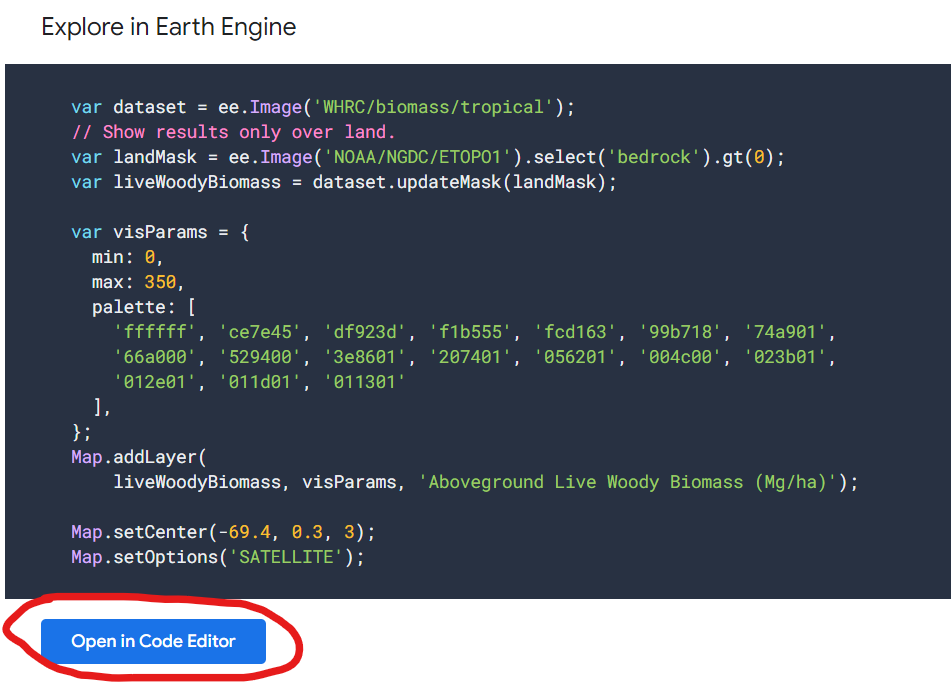
\includegraphics[width=3.17in,height=\textheight]{Validar cuenta.png}

}

\end{figure}

\begin{enumerate}
\def\labelenumi{\arabic{enumi}.}
\setcounter{enumi}{2}
\tightlist
\item
  De clic en \textbf{Open in Code Editor}, esto abrirá una nueva pestaña
  en el navegador, siga las instrucciones hasta obtener la siguiente
  imagen.
\end{enumerate}

\begin{Shaded}
\begin{Highlighting}[]
\NormalTok{knitr}\SpecialCharTok{::}\FunctionTok{include\_graphics}\NormalTok{(}\StringTok{"Validar cuenta2.png"}\NormalTok{)}
\end{Highlighting}
\end{Shaded}

\begin{figure}[H]

{\centering 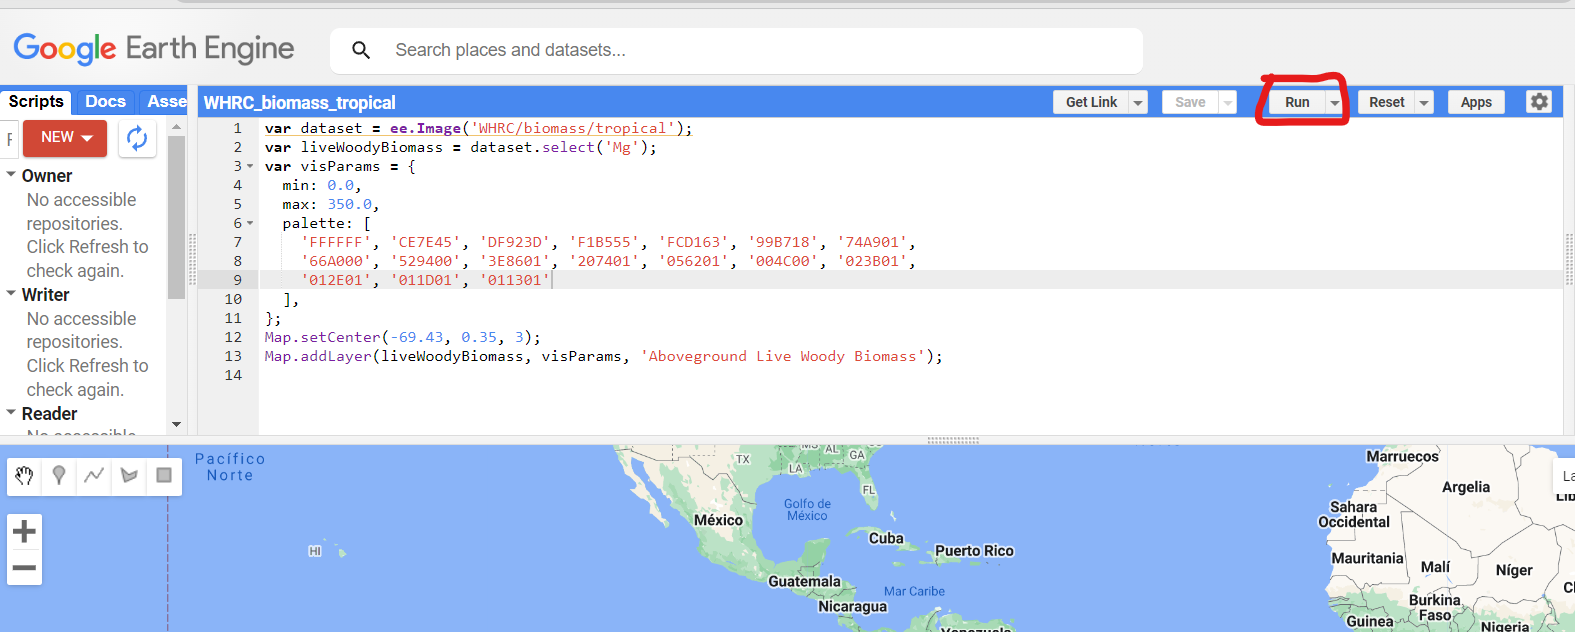
\includegraphics[width=5.25in,height=\textheight]{Validar cuenta2.png}

}

\end{figure}

\begin{enumerate}
\def\labelenumi{\arabic{enumi}.}
\setcounter{enumi}{3}
\tightlist
\item
  En la pestaña anterior, identifique el botón \textbf{Run}, presiona
  para obtener la imagen.
\end{enumerate}

\begin{Shaded}
\begin{Highlighting}[]
\NormalTok{knitr}\SpecialCharTok{::}\FunctionTok{include\_graphics}\NormalTok{(}\StringTok{"Validar cuenta3.png"}\NormalTok{)}
\end{Highlighting}
\end{Shaded}

\begin{figure}[H]

{\centering 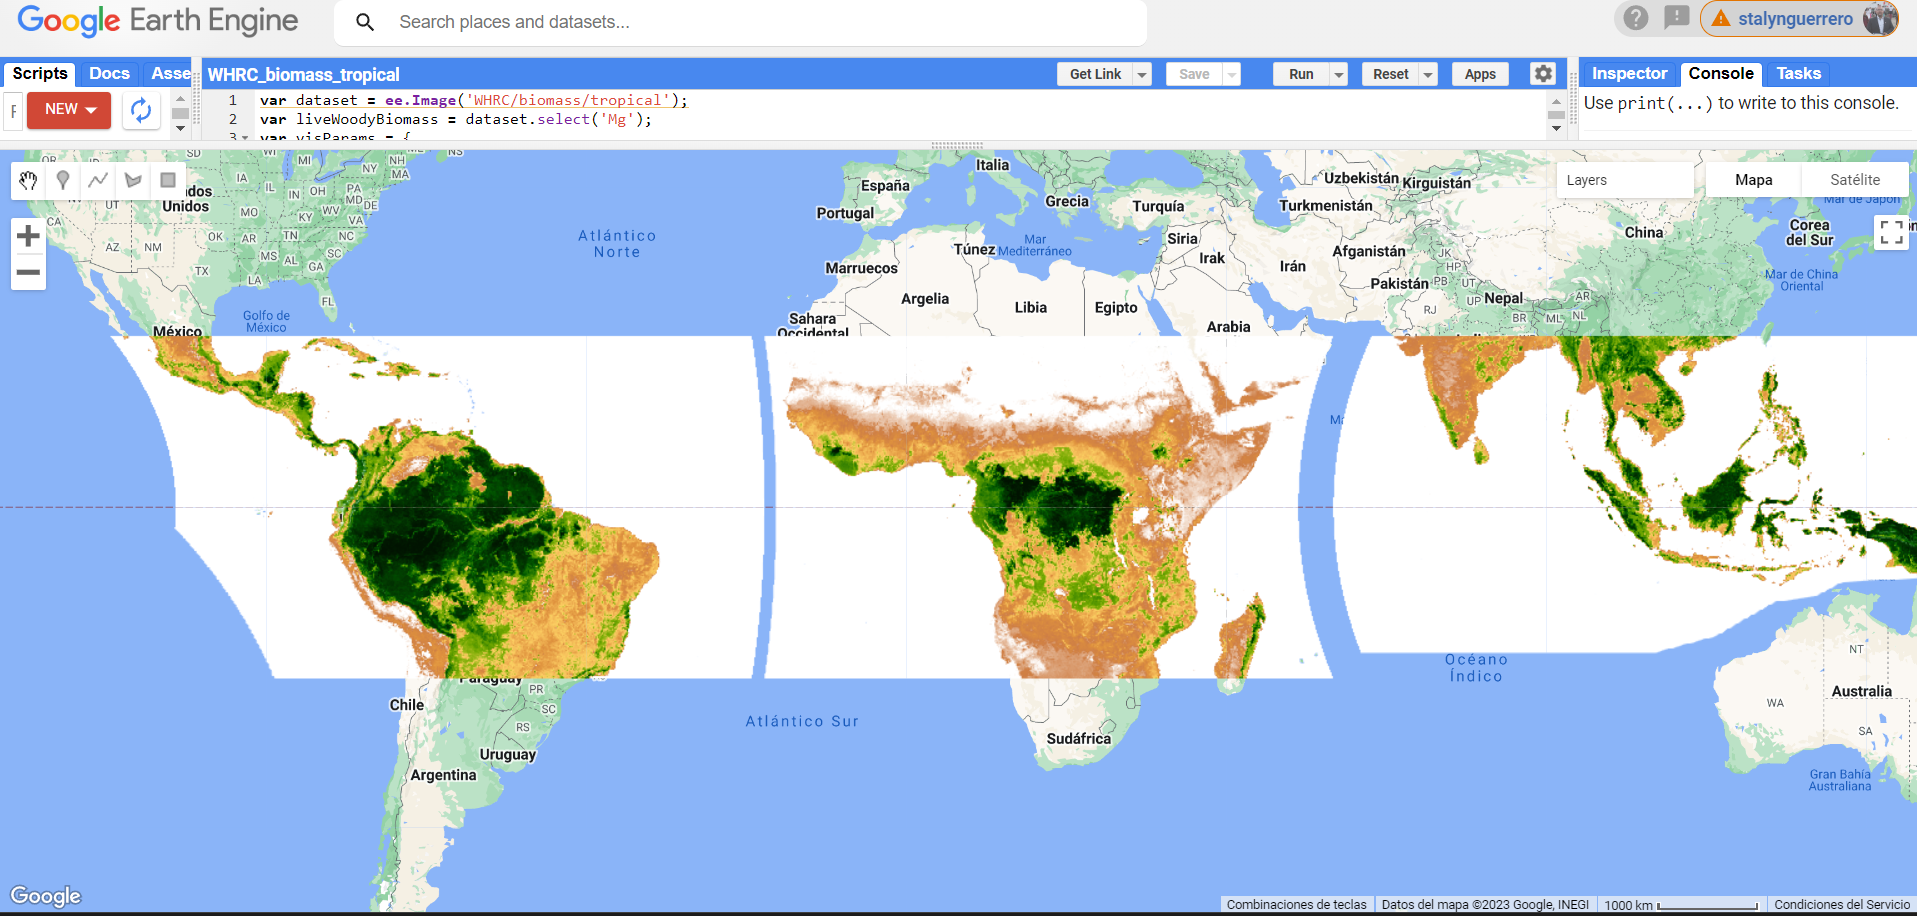
\includegraphics[width=6.39in,height=\textheight]{Validar cuenta3.png}

}

\end{figure}

\textbf{Nota}: Repetir el proceso hasta obterner el resultado indicado.



\end{document}
